\documentclass[../main.tex]{subfiles}

\begin{document}

\chapter{June $16^{th} / 2025$}
\label{ch:tufte-design}

\newthought{Cardiovascular Diseases and the Role of Missense Variants}

\subsection*{Missense Variant} 

single nucleotide change in DNA resulting in another AA incorporated in $x$ protein. Possible outcome  $\rightarrow$ \textit{benign} or \textit{severly disruptive} which often leads to alteration of protein structure and thus function.

In cardiogenetics, missense variants are a common in mechanism of disease particularly for \textit{inherited heart muscle and rhythm disorder}.

\vspace{0.2cm}

\textbf{Key examples:} 

\vspace{0.2cm}

\textbf{Hypertrophic Cardiomyopathy (HCM):} Thickening of the heart muscle. \textbf{MYH7} amd \textbf{MYBPC3} are the most common involved genes which encode proteins of the sarcomere (heart's contractile unit). The variants often lead to an altered protein that gets incorporated into the sarcomere and disrupts its function often through a \textbf{Dominant-Negative Effect} where the abnormal protein interferes with the function of the normal protein from the other allele.

$\blacktriangleright$ As noted in ACMG/AMP, simple loss-of-function (null) variants in many of such genes are more likely to be benign. Therefore, presence of $x$ faulty component (missense variant) in the machine contributes to its abnormal behaviour \textit{not} the lack of such component. 

\vspace{0.3cm}

\textbf{Dilated Cardiomyopathy (DCM):} Enlarged and weakened left ventricle. Missense variants in genes encoding proteins of the sarcomere (e.g., TTN), cytoskeleton, nuclear envelop are major the major cause \textit{but} loss-of-function variants can also cause DCM. These variants can compromise the structural integrity and force-generating capacity of the heart muscle cells

\vspace{0.3cm}

\textbf{Arrythmogenic Cardiomyopathy (ACM):} Tissue is replaced by fatty and fibrous tissue which lead to arrhythmias. Often caused by missense variants in genes that encode \textbf{desmosomal} protein (e.g., PKP2, DSG2, DSP) which are essential for holding heart cells together. A single AA change can disrupt cell-cell junctions $\rightarrow$ cell death / disease.

\vspace{0.3cm}

\textbf{Cardiac Channelopathies:} Group of disorders caused by mutations in genes encoding cardiac ion channels that control the heart's electrical activity. Their primary mechanism is often missense variants. 

\hrulefill

\newthought{Genetics of myocardial interstitial fibrosis in the human heart and association with disease} \cite{Nauffal2023}

\hrulefill

\section{Myocardial Interstitial Fibrosis:}
Pathological scarring of heart muscle. Excessive deposition of extracellular matrix proteins (e.g., collagen) that lead to cardiac stiffness, impaired function, and ultimately, heart failure.

\subsection{Monogenetic Causes:}
\textit{These are typically rare variants with a large effect size}

\vspace{0.2cm}

\textbf{Sarcomeric Genes in Hypertrophic Cardiomyopathy (HCM)} Most common genetic heart disease. A major cause are mutations that code for the sarcomere (contractile unit).

\vspace{0.2cm}

\textit{Frequently implicated genes:}

\begin{itemize}
    \item \textbf{MYH7 (Myosin Heavy Chain 7):} Encodes $\beta$-myosin heavy chain (motor protein for muscle contraction)
    \item \textbf{MYBPC3 (Myosin Binding Protein C, Cardiac):} Encodes protein that regulate the contraction and relaxation of the heart muscle
\end{itemize}

Other sarcomere-related genes are TNNT2, TNNI3. These mutations are thought to initiate a cascade that results in fibrosis. The presence of such mutations is strongly associated with a greater extent of myocardial fibrosis

\section{Polygenic Risk: Cumulative Effect} 

For a large portion of the population the rick of developing myocardial fibrosis is not tied to a single faulty gene but rather to the combined influence of many common genetic variants. GWAS have identified loci associated with an increased risk of fribrosis. Such variants are linked to a variety of biological processes that when altered can promote a pro-fibrotic environment in the heart.

\begin{itemize}
    \item \textbf{Glucose Transpose:} Variants in \textbf{SLC2A12} may alter energy metabolism within the heart 
    \item \textbf{Iron Homeostasis:} \textbf{HFE} and \textbf{TMPRSS6} suggest a link between iron regulation and cardiac scarring
    \item \textbf{Oxidative Stress:} \textbf{CAMK2D} variant is involved in calcium signaling which is critical for cardiomyocyte function and survival
    \item \textbf{Tissue Repair and Remodelings:} \textbf{ADAMTSL1} and \textbf{VEGFC} play roles in how the extracellular matrix is maintained and repaired
    \item \textbf{Chromatin Remodeling:} \textbf{SMARCB1} variants have been linked to an increased risk of fibrosis. Decreased expression of it can lead to an exaggerated response to fibrotic stimuli.
\end{itemize}

$\blacktriangleright$ Regardless of the trigger (monogenic or polygenic), multiple signaling pathways are implicated in downstream process of fibrosis. Genetic variations tend to converge on such pathways $\rightarrow$ Amplification Fibrotic Response.

\begin{figure}[h!]
    \begin{minipage}[t]{0.48\textwidth}
        \centering
        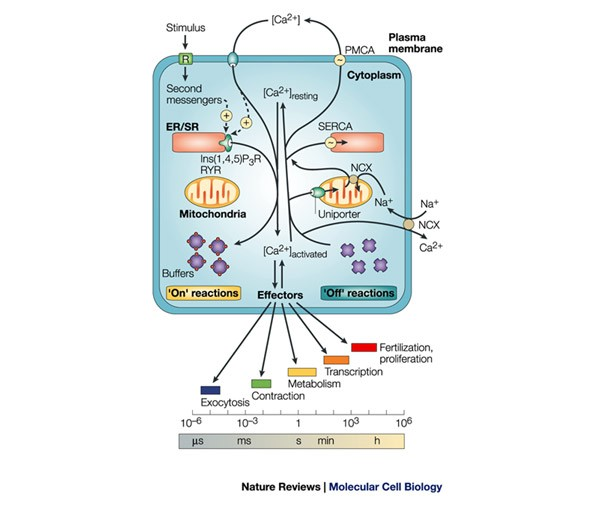
\includegraphics[width=\linewidth,height=5cm,keepaspectratio,valign=t]{files/images/calcium_path.jpg}
        \caption{Calcium Pathway \cite{Berridge2003}}
        \label{fig:calcium_path}
    \end{minipage}
    \hfill % Adds horizontal space between the minipages
    \begin{minipage}[t]{0.48\textwidth}
        \centering
        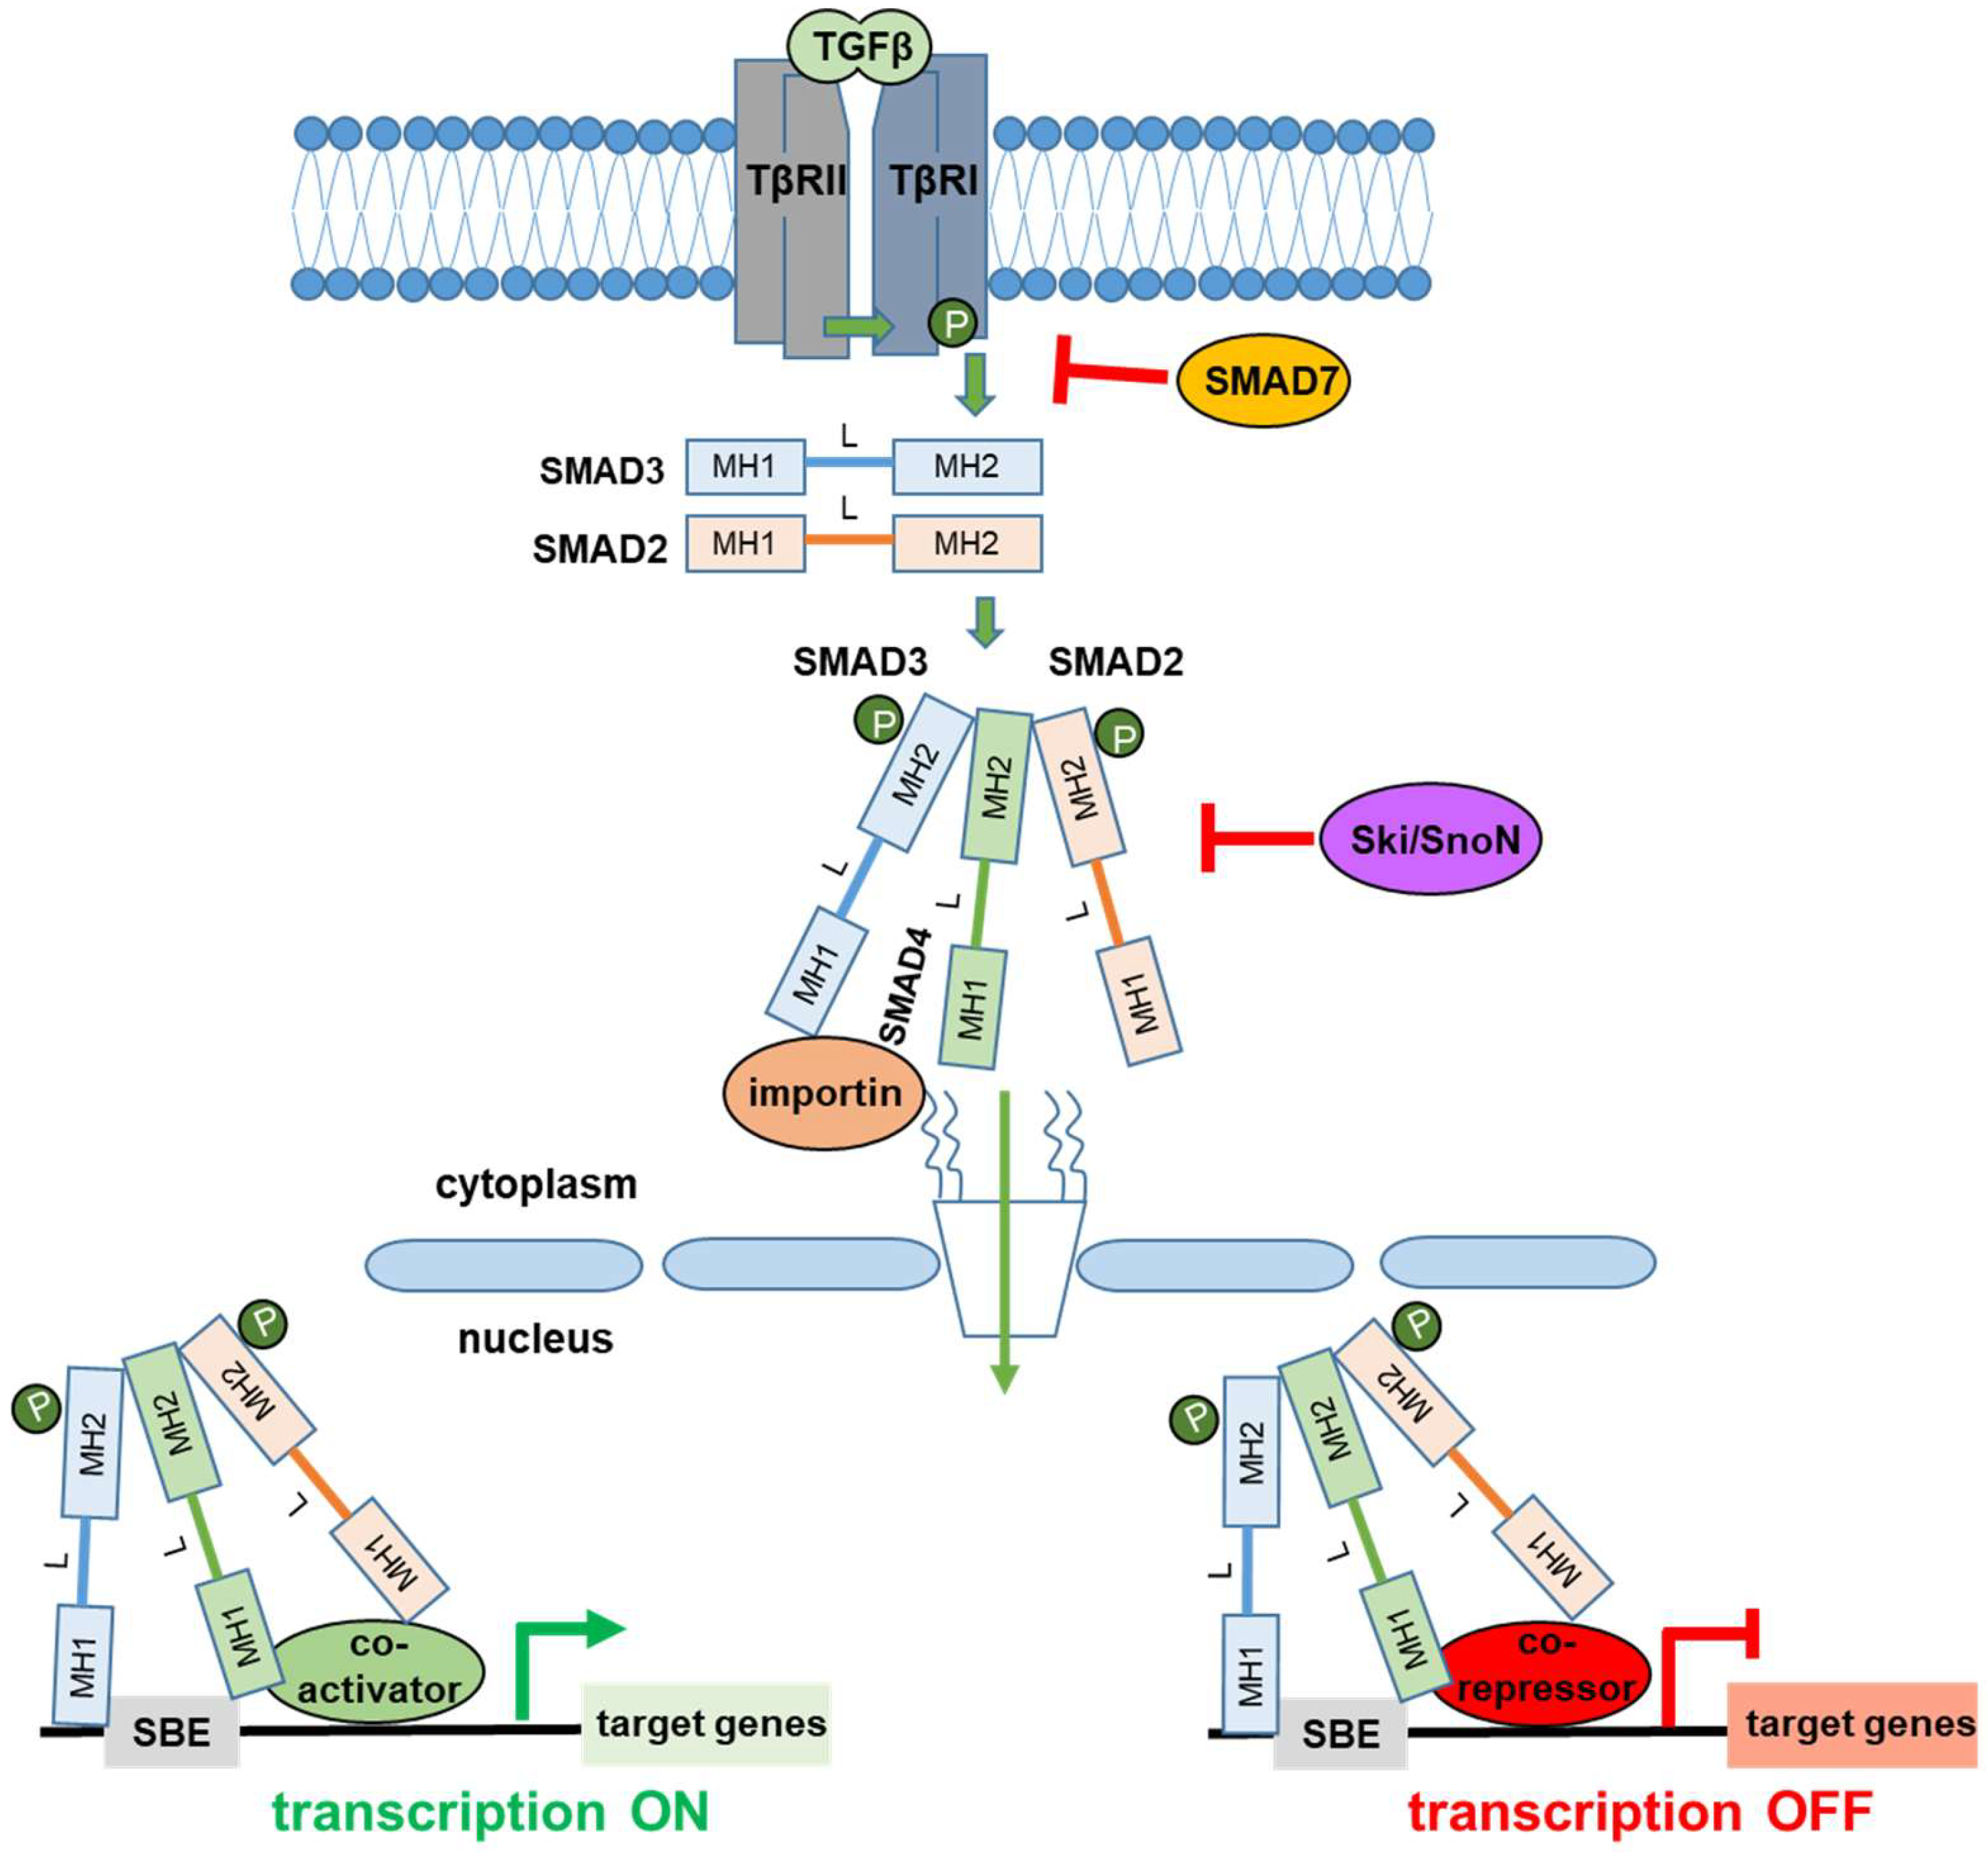
\includegraphics[width=\linewidth,height=5cm,keepaspectratio,valign=t]{files/images/tgf_path.png}
        \caption{TGF Pathway \cite{cells8090960}}
        \label{fig:tgf_path}
    \end{minipage}
    \centering
    \caption{Signaling pathways: Calcium and TGF} % Overall caption for the figure
    \label{fig:combined_pathways}
\end{figure}

\vspace{0.5cm}

Authors \textbf{goal} is to overcome limitation in understanding genetic basis of \textbf{myocardial interstitial fibrosis} using ML to quantify fibrosis from \textit{cardiac magnetic resonance imaging \textbf{(CMRI)}} (UK biobank cohort) then identify novel genetic pathways in the disease.

\section{U-Net with DenseNet-121 encoder}
Symmetric encoder-decoder structure. Designed to capture context and localization 

\subsection{DenseNet-121 Encoder} 

\textbf{Input} image $\rightarrow$ hierarchical feature representations at different spatial scales.

\begin{itemize}
    \item \textbf{Cmmposite Layer Function ($H_l$)}

    Let $x_{l-1}$ output preceding layer: $x'_l = Conv(ReLU(BN(x_{l-1})))$
    \begin{itemize}
        \item \textbf{Batch Normalization (BN)} normalizes input $z$, scales, shifts it. For input feature map $z$:

        \[
            BN(z) = \gamma (\frac{z-\mu_{batch}}{\sqrt{\sigma^2_{batch}+\epsilon}}) + \beta
        \]

        where $\mu$ and $\sigma^2$ pertain to mini-batch. $\beta$is shifting parameter, $\gamma$ is learning rate
    \end{itemize}
    \item \textbf{Dense Connectivity}
    
    Output of $l$ is $x_l = H_l([x_0,x_1,...,x_{l-1}])$ composite function $H_l$ is applied to \textbf{concatenation} of feature maps along channel dimension (e.g., $k_0 + (l+1) * k$ channels for $l$)

    \item \textbf{Transition Layers} 

    [Between dense blocks] Used to control complexity and \textit{downsample spatial dimensions of feature maps}.
    \begin{itemize}
        \item $1*1$ convolution to reduce number of feature maps
        \item $2*2$ avg. pooling layer to halve height/width of feature map

        \[
        x_{trans}=AvgPool(Conv_{1*1}(x))
        \]
    
    \end{itemize}
    
\end{itemize}

\section{U-Net Decoder and Skip Connections}
Overall framework for segmentation. Input is output from encoder. 

\begin{itemize}
    \item \textbf{Encoder-Decoder Symmetry}
    The U-Net has $2$ paths:
    \begin{itemize}
        \item  \textbf{Encoder:} DenseNet-121 \textbf{output} from different levels: $e_1, e_2, e_3, e_4$
        \item The \textbf{Decoder} symmetrically reconstructs the spatial resolution to produce segmentation map
    \end{itemize}

    \item \textbf{Upsampling (Transposed Convolution (or deconvolution)}

    let $d_i$ be the feature map at level $i$ in the decoder. The unsampled feature map $u_i$: $u_i = TransConv(d_i)$

% Combined Focal and Dice Loss Function
% L(p, g) is the total loss for a prediction 'p' and ground truth 'g'.
% It is a weighted sum controlled by the hyperparameter \alpha.
\begin{equation}
    L(p, g) = \alpha \cdot L_{\text{focal}} + (1 - \alpha) \cdot L_{\text{dice}}
\end{equation}

% --- Focal Loss Component ---
% L_focal focuses training on hard-to-classify examples.
% The focusing parameter \gamma >= 0 adjusts the rate at which easy examples are down-weighted.
\begin{equation}
    L_{\text{focal}} = - (1 - p_t)^\gamma \log(p_t)
\end{equation}
% where p_t is the model's estimated probability for the ground truth class 'g'.
\[
p_t =
\begin{cases}
    p & \text{if } g = 1 \\
    1 - p & \text{otherwise}
\end{cases}
\]

% --- Dice Loss Component ---
% L_dice is calculated as 1 minus the Dice Coefficient. It is effective for class imbalance.
% The sums are over all pixels 'i'.
% The term \epsilon is a small smoothing factor to prevent division by zero.
\begin{equation}
    L_{\text{dice}} = 1 - \frac{2 \sum_{i} (p_i \cdot g_i) + \epsilon}{\sum_{i} p_i^2 + \sum_{i} g_i^2 + \epsilon}
\end{equation}
    
\end{itemize}


\begin{figure}[h!] % [h!] tries to place the figure "here"
    \centering % Centers the figure horizontally
    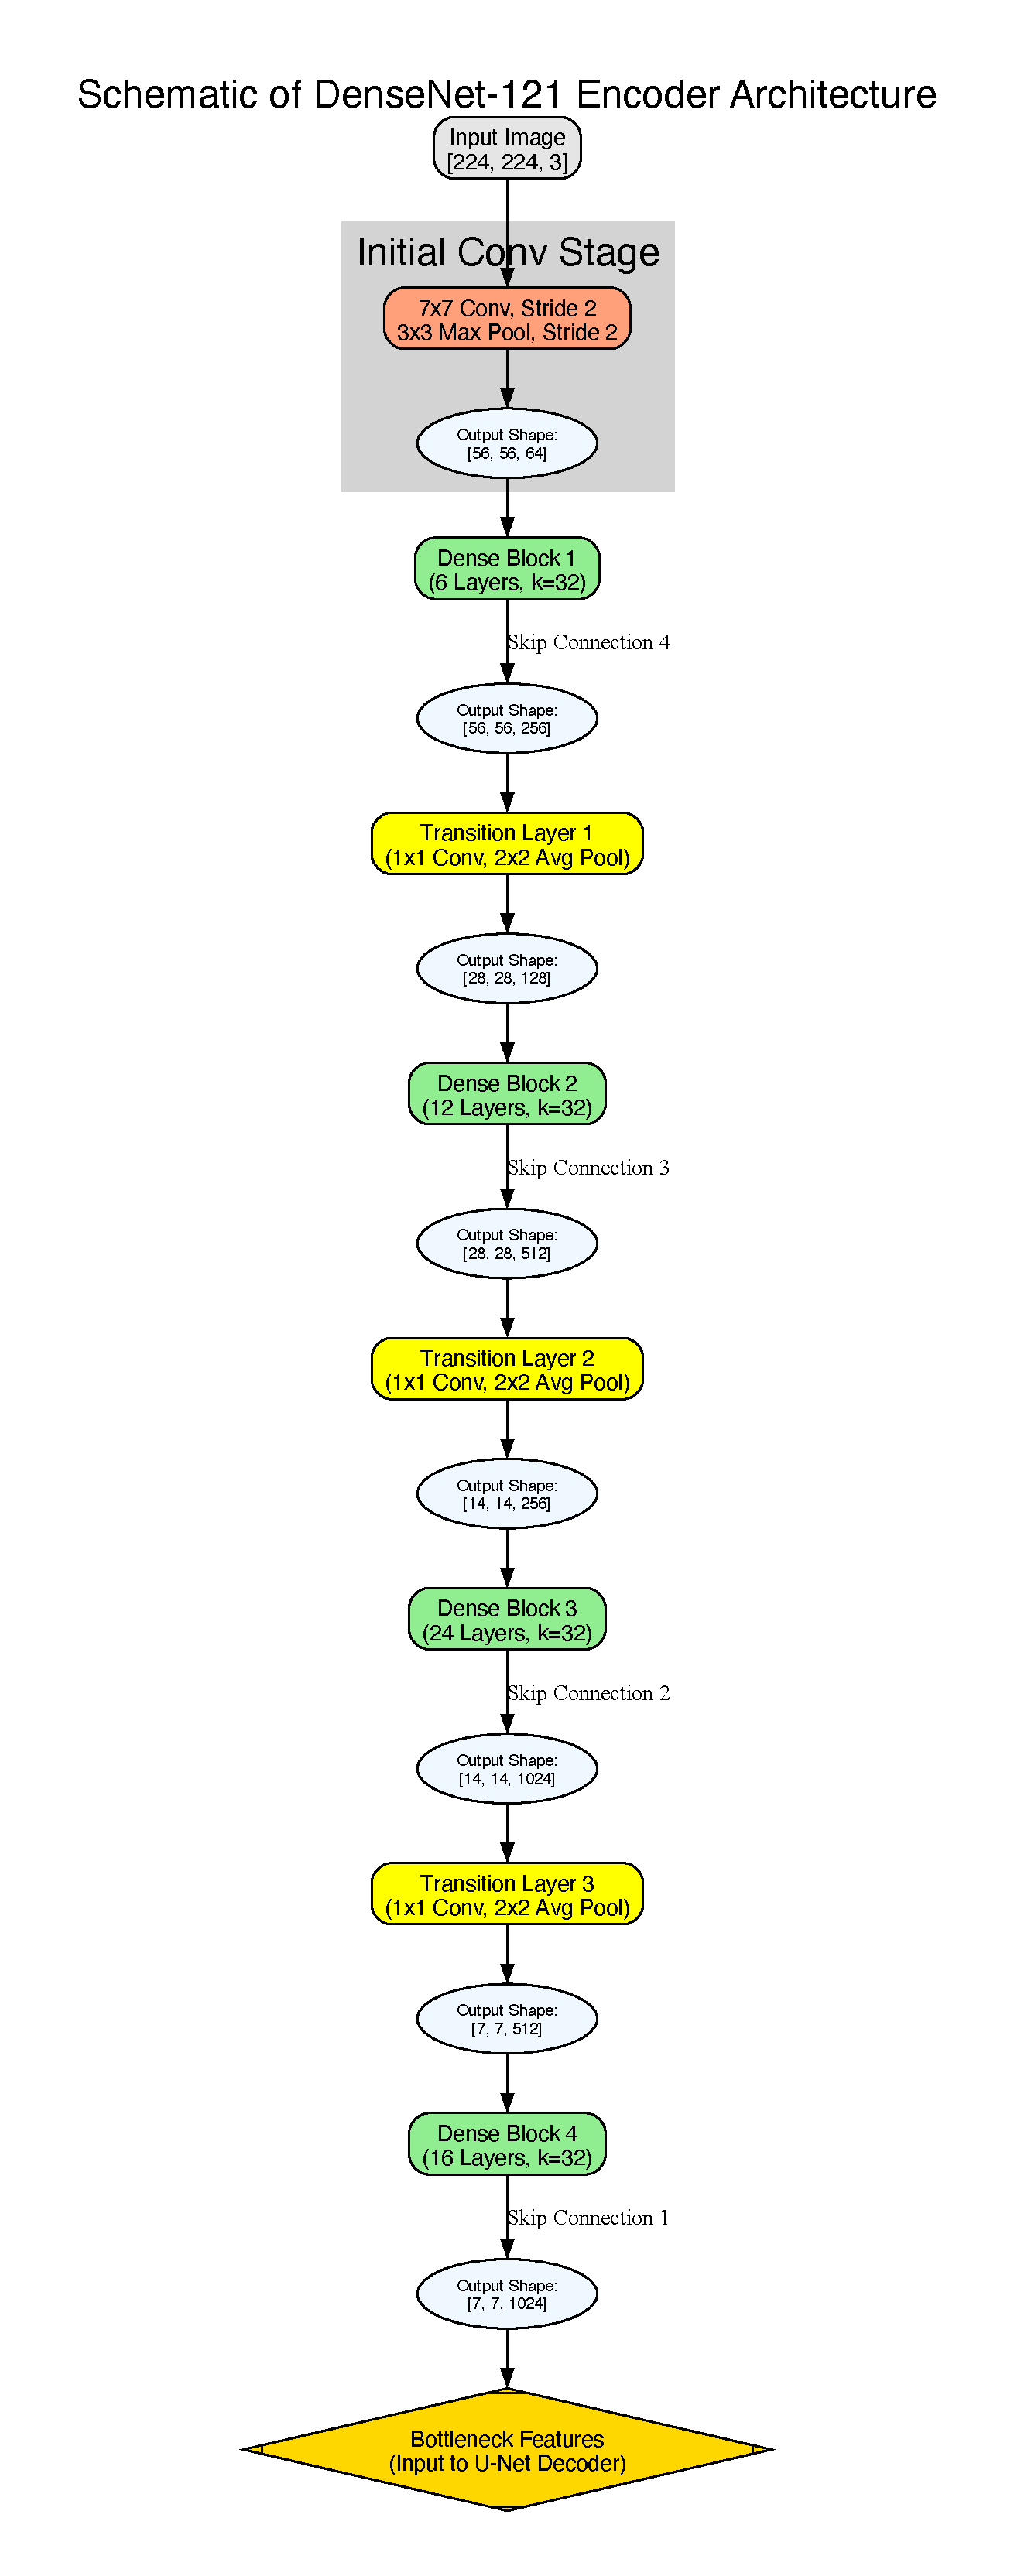
\includegraphics[width=0.8\textwidth]{densenet121_structure.pdf} % Include your PDF graph
    \caption{Model structure.} % Caption for the figure
    \label{fig:my_pdf_graph} % Label for cross-referencing
\end{figure}


\end{document}